
\begin{frame}{Bonnes pratiques dans le numérique}{Conseils 45-49/115}
\begin{block}{Réduire les accès au DOM via JavaScript}
Assigner le nœud dans des variables évite de retraverser l’arbre à chaque manipulation du document.
\end{block}

\begin{block}{Utiliser tous les niveaux de cache du CMS}
Utiliser la granularité du CMS réduit les ressources consommées.
\end{block}

\begin{block}{Optimiser et générer les médias avant importation sur un CMS}
 FFmpeg, Any Video Converter, Xnview, Gimp, Inskape, PDFedit...
\end{block}

\begin{block}{Encoder les sons en dehors du site web}
Un serveur web n’est pas optimisé pour le (ré)encodage des fichiers audio.
\end{block}

\begin{block}{Mettre en cache les données calculées souvent utilisées}
Par exemple, Mettre en cache les jetons d'accès en OAuth2 et son délai d'expiration évite des appels inutiles au serveur d'autorisation.
\end{block}


\end{frame}


\begin{frame}{Bonnes pratiques dans le numérique}{Conseils 50-51/115}
\begin{block}{Supprimer tous les warning et toutes les notices}
Les warnings et notices ralentissent les serveurs d’applications tels que PHP, car ces derniers doivent retracer l’origine des erreurs et inscrire dans les différents journaux système les messages expliquant les problèmes rencontrés.
\begin{figure}
    \centering
    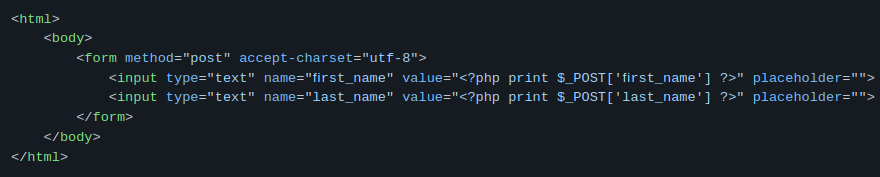
\includegraphics[scale=0.3]{chapitre2/wdd5/fig/c1.png}
\end{figure}
\end{block}

\begin{block}{Éviter d'effectuer des requêtes SQL à l’intérieur d’une boucle}
 Ces requêtes consomment inutilement des cycles CPU, de la mémoire vive et de la bande passante.
\end{block}

\end{frame}


\begin{frame}{Bonnes pratiques dans le numérique}{Conseils 52-53/115}
\begin{block}{Ne se connecter à une base de données que si nécessaire}
HikariCP est un pool de connexions JDBC solide et performant. Il est intégré dans SpringBoot.

Dans les cas où il n'y a pas de pool de connexion, réutiliser une connexion et ne pas ouvrir/fermer une nouvelle connexion à chaque requête.
\end{block}

\begin{block}{Optimiser les requêtes aux bases de données}
 Ces requêtes consomment inutilement des cycles CPU, de la mémoire vive et de la bande passante.

\end{block}

\begin{minipage}[b]{0.5\linewidth}
\begin{alertblock}{Ne pas écrire}
\begin{figure}
    
\includegraphics[scale=0.4]{chapitre2/wdd5/fig/c2.png}
    \centering
\end{figure}
 \end{alertblock}
\end{minipage}\hfill
\begin{minipage}[b]{0.5\linewidth}
\begin{exampleblock}{Mais plutôt}
\begin{figure}
    
\includegraphics[scale=0.4]{chapitre2/wdd5/fig/c3.png}
    \centering
\end{figure}
 \end{exampleblock}
\end{minipage}\hfill

\begin{figure}
    \centering
    
\includegraphics[scale=0.4]{chapitre2/wdd5/fig/c4.png}
\end{figure}
\end{frame}



\begin{frame}{Bonnes pratiques dans le numérique}{Conseils 54-56/115}
\begin{block}{Éviter le transfert d'une grande quantité de données pour réaliser un traitement}
Utiliser des  procédures stockées (SQL Server, MySQL, PostgreSQL, etc.).
\end{block}

\begin{block}{Minifier les fichiers CSS, JavaScript, HTML et SVG}

Minifier CSS, Javascript, HTML et SVG permet de supprimer les espaces inutiles, les commentaires des développeurs, les sauts de ligne, les délimiteurs de blocs et ainsi réduire leur taille.

\begin{itemize}
    \item CSS: cssnano, csso ou clean-css
    \item Javascript: Terser, UglifyJS ou Babel-minify
    \item HTML: htmlnano, HTMLMinifier
    \item SVG: SVGO, minify-xml ou équivalent
\end{itemize}

\end{block}

\begin{block}{Compresser les fichiers CSS, JavaScript, HTML et SVG}
Utiliser GZIP coté serveur, ou BROTLI côté client.
\end{block}
\end{frame}

\begin{frame}{Bonnes pratiques dans le numérique}{Conseils 57-59/115}
\begin{block}{Combiner les fichiers CSS et JavaScript}
\begin{itemize}
    \item Dans Wordpress, le plugin Autoptimize, combiner les fichiers CSS.
    \item Avec Webpack, le plugin webpack-merge-and-include-globally facilite la fusion des fichiers CSS et Javascript.
\end{itemize}
\end{block}

\begin{block}{Optimiser les images}
Outils pour réduire au minimum le poids des images :
    SQUOOSH,
    CLOUDINARY,
    ImageMagick,
    PngCrush,
    JpegTran
\end{block}

\begin{block}{Optimiser la taille des cookies}
Supprimer un cookie lorsqu’il n’est plus utile en précisant une durée d’expiration nulle ou négative.


\begin{figure}
    \centering
    
\includegraphics[scale=0.5]{chapitre2/wdd5/fig/c5.png}
\end{figure}
\end{block}
\end{frame}


\begin{frame}{Pause débunkage }{Triangle de l'inaction}
\begin{figure}
    \centering
    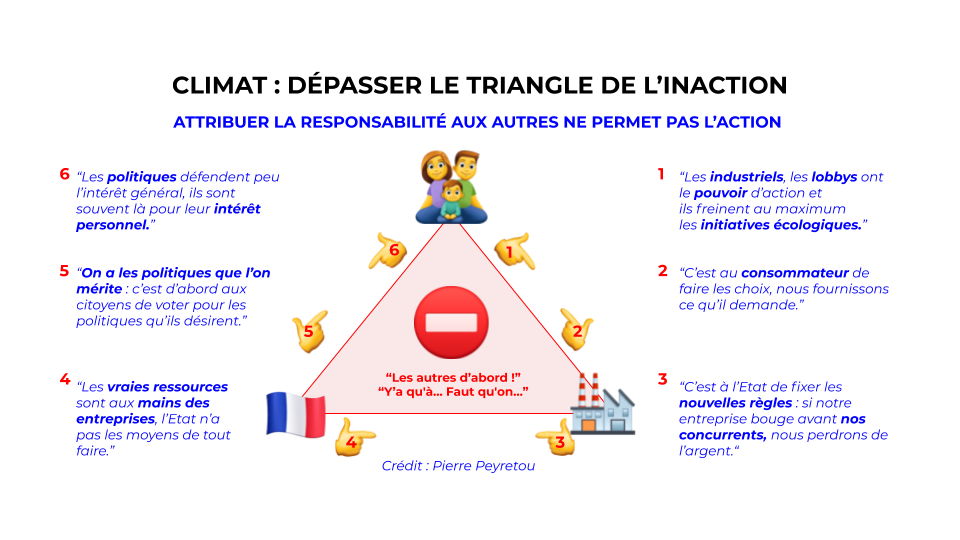
\includegraphics[scale=0.35]{Feathergraphics/[Outils Méthodo] Triangle de l'inaction.png}
\end{figure}
\end{frame}